\documentclass[a4paper,11pt]{article}
\usepackage{graphicx}
\usepackage[T1]{fontenc}
\usepackage[utf8]{inputenc}
\usepackage{lmodern}
\usepackage{float}
\usepackage[lofdepth,lotdepth]{subfig}
\usepackage[english]{babel}
\usepackage[margin=1in]{geometry}
\usepackage{wrapfig}
\usepackage{amsmath}

\title{Statistical Mechanics Project}
\author{Adam Lamson\\
Department of Physics\\
University of Colorado Boulder\\
\texttt{Adam.Lamson@colorado.edu}}
\date{4/29/16}

\begin{document}

\maketitle

\begin{center}
\end{center}

\tableofcontents

\begin{abstract}
    In this project we simulate a 2-D finite Ising model with periodic boundary conditions and a square unit cell. The Ising Model Hamilitonian is given by
    \begin{equation}
        \mathcal{H} = -J \sum_{\langle ij \rangle} s_i s_j - H\sum_i s_i
    \end{equation}
    where $s_i$ represents the spin of particle i with a value of $\pm1$, $J$ is the strength of the coupling between adjacent particles, and $H$ is the strength of external magnetic field. In the canonical enssemble a system of V\footnote{$V=L*L$ where L is the number of particle per side of a unit cell.} particles can be defined by the values of $J$, $H$, and kT\footnote{The temperature of the ensemble multiplied by the boltzmann factor. We will simply refer to this as T for the rest of the paper.}. From these we can determine quantities such as the energy, magnetization, and susceptibility of each system. The energy, $E$, simply uses the above Hamilitonian while the magnetization is simply defined as 
    \begin{equation}
        M = \sum_i s_i
    \end{equation}
The susceptibility of the system is then defined as 
    \begin{equation}
        \chi = \frac{\partial M}{\partial H}\bigg\vert_T 
    \end{equation}

    In 2-D there is an analytical solution for the Ising Model, however, this proves overly complicated most of the time. An easier approach in the modern day is to use very simple simulation techniques to obtain the above calculated values. I created a python program(attached) that implemented both the heat bath and metropolis algorithm to thermalize a system of volume V. To find the critical temperature, $T_c$, a logarithmic slice of temperatures was taken from .01 to 100 with $J=1$ and $H=0$. Once the two values that showed the transition from highly ordered to disordered was identified a linear slice was taken to find critical temperature to higher and higher degrees of accuracy. This showed strong correlation to the known value of $T_c \approx 2.269$. Anti-ferromagnetic behavior was seen for negative values of $J$ but most measurements were conducted with $J=1$.

\end{abstract}

\section{The 2-dimensional Ising model}

    \subsection{Thermalization of $E$ and $M$}

        \paragraph{Initial Tests}We begin by showing that at low temperatures systems will have spins that are all strongly correlated while at higher temperatures this correlation fades.

        \begin{figure}[H]
            \centering
            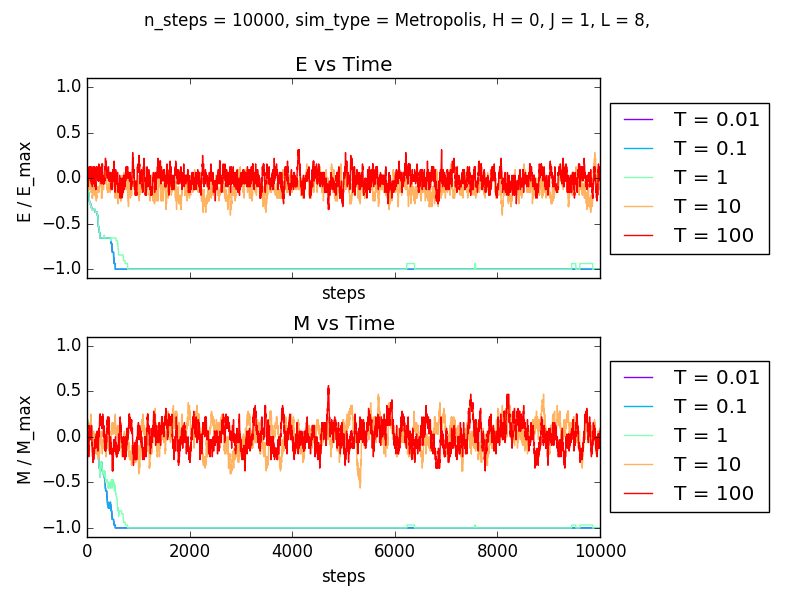
\includegraphics[width=.75\textwidth]{Graphs/Large_Temp_slice.png}
            \caption{Time evolution of system of 64 particles showing the different behaviors at various temperatures. E = Energy and M = Magnetization} 
        \end{figure}

        As expected we see two regimes emerge with $T \le 1$ showing a steady state of lowest energy and relatively constant magnetization while $T \ge 10$ random distributions around 0 for both magnetization and energy. From this we can deduce that the critical Temperature, $T_c$, where systems will go from having spins correlated to being uncorrelated in orientations, exists between 1 and 10. 


        \paragraph{Finding $T_c$} We can look at the average energy and magnetization of runs at various temperatures to find the transition and thus the critical temperature.
        
        \begin{figure}[H]
            \centering
            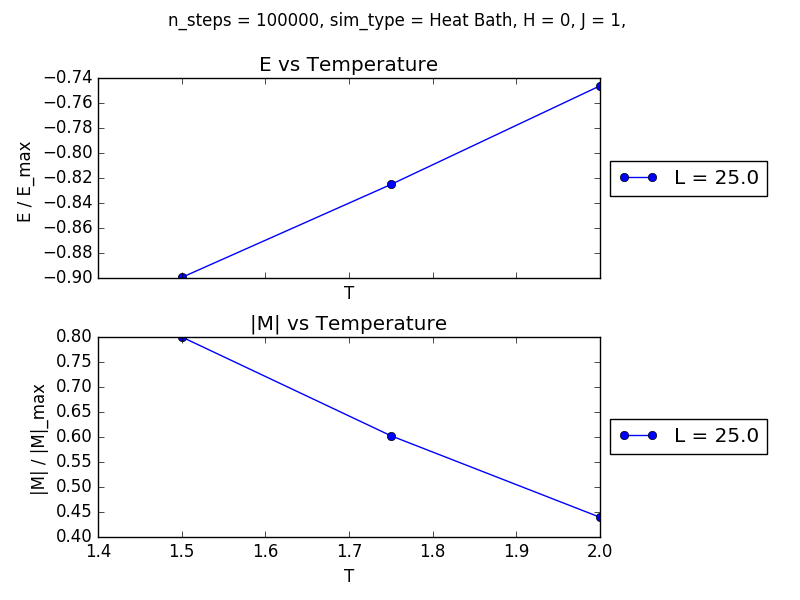
\includegraphics[width=.75\textwidth]{Graphs/Find_Tc_slice_2.png}
            \caption{ Absolute value of the magnetization and average energy plotted against temperature of the system. Multiple sized systems were compared to see if volume of the system showed different critical temperatures.}
        \end{figure}

        In Figure 2 we can see that transition of the system takes place somewhere between $2.25$ and $2.75$. Online literature indicates that $T_c \approx 2.2693$. For these systems the transition seems to take place rather smoothly over a temperature range of around $.5$. However, this behavior might change with increased system size.

    \subsection{Dependence on $H$}

    \subsection{Tunneling}

    \subsection{Difference of Algorithms}


\section{Ising Fluctuations and Susceptibilities}

    \subsection{Correlations and Susceptibilities: Analytical}
        To calculate the average magnetization of the Ising Model we start with Helmholtz Free Energy defined as        
        \begin{equation}
            A=-\frac{1}{\beta}ln(Z)
        \end{equation}
        where $Z$ is the partition function, $\sum_i e^{-E_i\beta}$ and $E_i$ is the energy calculated from a particular system $i$ using the Hamiltonian, $\mathcal{H}$. Taking the partial derivative of $A$ with respect to $H$ at a constant temperature then gives
        \begin{equation}
        \frac{\partial A}{\partial H}\bigg\vert_T = \frac{-1}{\beta Z}\frac{\partial{Z}}{\partial{H}}\bigg\vert_T =-\frac{1}{\beta Z} \sum_i( e^{-E_i\beta} (-\beta \frac{\partial{E_i}}{\partial{H}}\bigg\vert_T))
        \end{equation}

        From the definition of the Hamiltonian we see that
        \begin{equation}
            \frac{\partial{E_i}}{\partial{H}}\bigg\vert_T = -\sum_j s_j = -M_i
        \end{equation}
        the negative value of the magnetization for configuration $i$. This means

        \begin{equation}
            -(\frac{\partial A}{\partial H}\bigg\vert_T) = \frac{1}{Z}\sum_i( M_i e^{-E_i\beta}) = \langle M \rangle
        \end{equation}
        by the definition for averages in the canonical ensemble. Thus we see that the negative partial derivate of the Helmholtz Free Energy with respect to the applied $H$ field gives us the average magnetization at a temperature, T. We can the fine the susceptibility in terms of fluctations using the formula, $\chi = (\partial{\langle M \rangle}/\partial{H})|_T$. Using our results and identities from above
        
        \begin{equation}
        \begin{split}
            \frac{\partial \langle M \rangle}{\partial H}\bigg\vert_T &= \frac{\partial}{\partial H}(\frac{1}{Z}\sum_i( M_i e^{-E_i\beta}) \\
            &= \frac{1}{Z^2}(Z \sum_i( M_i e^{-E_i\beta} \frac{\partial{E_i}}{\partial{H}}\bigg\vert_T) - \sum_i( M_i e^{-E_i\beta}\frac{\partial{Z}}{\partial{H}}\bigg\vert_T))\\
            &=  \frac{1}{Z} \sum_i\beta M_i^2 e^{-E_i\beta} - \frac{1}{Z^2} (\sum_i M_i e^{-E_i\beta})(\sum_j \beta M_j e^{-E_j\beta})\\
            &= \beta (\langle M^2 \rangle - \langle M \rangle^2 ) = \chi
        \end{split}
        \end{equation}

        With this formula we can calculate the susceptibility of the our simulation using the variance and mean of the magnetization.

        %is the entropy which for this model is $S=k ln(\Omega) = kVln(2)$. If we take the partial j 

    \subsection{Correlations and Susceptibilities: Numerical}

    \subsection{Low Temperature Expansion for the Magnetization}
        In a system with a $T < T_c$ most of the spins will be aligned in the same orientation. The energy cost for taking a spin and flipping it to oppose its neighbors is
        \begin{equation}
            E_{flip} = E_{after} - E_{before} = 8J
        \end{equation}
        
        %Show graph with single fluctuations
        We can predict what the average magnetization of system will be for a given temperature below the critical value.

    \subsection{High Temperature Expansion for the Magnetization}
        At high temperatures $\langle M \rangle \rightarrow 0$. This turns our previous formula into

        \begin{equation}
            \lim_{\beta\to0} \chi = \beta \langle M^2 \rangle
        \end{equation}

        For a single spin in an external magnetic field we can write the energy and partition function as 

\section{Last part of the project}

    \subsection{Specific Heat: Analytical}
        As we did for the susceptability we can find an expression for the the specific heat using statistics produced by the simulation. First we use the definition of specific heat at a constant volume.
        \begin{equation}
            C_v = \frac{\partial{\langle E \rangle}}{\partial{T}}\bigg\vert_V = \frac{\partial\beta}{\partial T} \frac{\partial{\langle E \rangle}}{\partial{\beta}}\bigg\vert_V
        \end{equation}

        in the canonical ensemble we know the average energy is given as 

        \begin{equation}
        \langle E \rangle = - \frac{\partial}{\partial\beta}ln(Z) =\frac{1}{Z}\frac{\partial Z}{\partial \beta}
        \end{equation}

        Substituting this into equation ... 
        \begin{equation}
        \begin{split}
            C_v &= -\frac{\beta}{T}\frac{\partial}{\partial\beta}(-\frac{1}{Z}\frac{\partial Z}{\partial \beta})\\
                &= \frac{\beta}{T}(-\frac{1}{Z^2}(\frac{\partial Z}{\partial \beta})^2 +\frac{1}{Z}\frac{\partial^2 Z}{\partial \beta^2})\\
                &= \frac{\beta}{T}(-\langle E \rangle^2 +\frac{1}{Z}\sum_i E_i^2 e^{-E_i \beta})\\
                &= \frac{\beta}{T}(\langle E^2 \rangle - \langle E \rangle^2)
        \end{split}
        \end{equation}
        %$U$ is the average energy which in the canonical ensemble is given as

        %\begin{equation}
            %U = -\frac{\sum_i E_i e^{-E_i\beta}}{Z}
        %\end{equation}
        
        %where $E_i$ is calculated from the Hamiltonian, $\mathcal{H}$ from a particlular system configuration, $i$ and $Z$ is  the partion funtion $\sum_i e^{-E_i\beta}$.

    \subsection{Specific Heat: Numerical}

    \subsection{Finite Size Scaling}

\end{document}

